
%(BEGIN_QUESTION)
% Copyright 2010, Tony R. Kuphaldt, released under the Creative Commons Attribution License (v 1.0)
% This means you may do almost anything with this work of mine, so long as you give me proper credit

Sketch the necessary wires between instruments in this pictorial diagram so that the controller will receive a pressure measurement signal (4-20 mADC) from the loop-powered transmitter into its process variable (PV) input terminals, and the control valve will be actuated by the controller's 4-20 mA output signal coming from the manipulated variable (MV) terminals.  Be sure to include any necessary 120 VAC power sources and wires!

$$\includegraphics[width=15.5cm]{i00009x02.eps}$$


\vfil

This question is typical of those in the ``Pictorial Circuit Diagrams'' worksheet found in the {\it Socratic Instrumentation} practice worksheet collection, except that all answers are provided for those questions.  Feel free to use this practice worksheet to supplement your studies on this very important topic.

\underbar{file i00009}
\eject
%(END_QUESTION)





%(BEGIN_ANSWER)

This is a graded question -- no answers or hints given!

%(END_ANSWER)





%(BEGIN_NOTES)

$$\includegraphics[width=15.5cm]{i00009x01.eps}$$

%INDEX% Pictorial circuit review (analog signal wiring to process controller)

%(END_NOTES)


